\chapter{Design}
\label{chap:design}

%In order to begin construction of the artifact it is necessary to understand the domain in which it should operate. To motivate design decisions we need to understand the domain data, what kinds of queries that will be done on this data as well as the overall architecture of the system. Once this understanding is reasonably adequate, designs decisions can be made with more confidence. However,  decisions should also take solution objectives into account. 

This chapter describes the design of the artifacts that are to be implemented in the form of prototypes. Some choices related to the design, like database schemas and choice of databases for the prototypes are motivated in more detail. Initially several candidate databases existed but these were narrowed down to two choices that were found to be interesting enough to move forward with. 

Through the review of related work, it has been established that non relational databases might be appropriate as a part of a solution to the identified problem of this thesis. However, it has also been suggested \cite{NoSQLSurvey} that the introduction of non relational storage should not replace current relational databases, but should instead work as a complement to them. We argue that a polyglot persistence solution is a natural approach to the identified problem. Implementing such a solution would then address objective 1, namely to physically separate live from stale data. Before implementation, a decision has to be made on what types of databases should be used as the underlying storage for the archive. If the only objective was data separation then the simplest choice would be to completely duplicate system data in its current form to a similar database. However, this does not take into account other objectives and would likely not solve the underlying problem. 

When selecting what databases to use we need address the issue of long running schema migrations. One way this could be addressed is by using a database with a flexible schema, capable of handling heterogeneous data. Said database should also have query capabilities that allow us to effectively address objective 2; the retainment of important queries.

In order for the archive system to scale naturally with the current level of data growth (objective 3), it is prudent to select a database with horizontal scaling. In addition to this, it would be highly beneficial with more efficient data compression than what is currently in use by the relational database of CIMS.

One NoSQL database and one relational database were selected to be used for the implementation of archive prototypes. They are described in more detail in the following sections.

%\section{MongoDB}
%The main motivation for choosing MongoDB as a candidate is its flexible data model along with custom indexes and %extensive query capabilities \cite{Catell}. As a comparison, a key-value store would be to constricting for the types %of queries that need to be supported by the archive as seen described in section~\ref{sec:usecases}. A document-store %has, at least in theory, the right mix between data model flexibility and query capabilities. Our intent with this %design choice is to evaluate the suitability of document-stores in general as a means to solve the identified problem. 

\section{Elasticsearch}
Elasticsearch \cite{elastic} is a NoSQL database classified as a search engine, with many similarities to a document store. Specifically, its data model and the ability to scale horizontally. The difference is mainly in query capabilities, which are optimized for full text search. However, supporting full text search comes at a price of higher demands on hardware. We believe this to be an interesting trade-off to consider, and a comparison between the other candidate database and Elasticsearch should yield useful practical information on how to proceed with the development of an archive solution after the study has been conducted.

\subsection{Data model for non-relational archive} \label{nosqlmodel}
With the domain description as a basis, the schema of the relational database in CIMS should be transformed to suit the strengths of the chosen NoSQL database. A level of denormalization is prudent since any relationship between collections in a document-store has to be implemented in application logic. However, no relationships at all would not be suitable for the types of queries that need to be supported. As such, the data model of the archive needs to be well designed. Given the use of document-stores and their data model, one natural change is to convert one to many relationships into lists of embedded documents. Another change is to denormalize all one to one relationships.

To illustrate the transformation process, we present a diagram in figure~\ref{fig:nosql} describing a proposed non relational schema for the archive. This can be compared to the original relational schema in figure~\ref{fig:sql}.

\begin{figure}[h!]
\centering
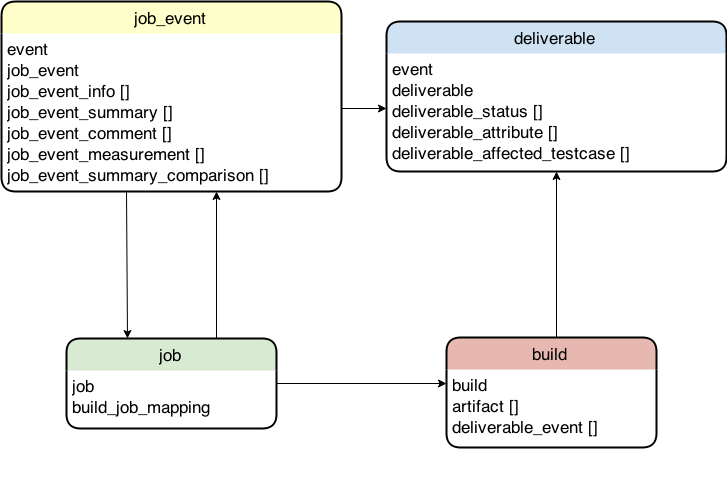
\includegraphics[scale=0.5]{figure/nosql.png}
\caption{Representation of the non-relational model. Bracket pairs represent a list of embedded documents.}
\label{fig:nosql}
\end{figure}

\section{TokuDB}
The second candidate database is MySQL using TokuDB \cite{tokudb} as the storage engine. Storage engines are software components that handle SQL operations without changing the overall architecture and interfaces of the database \cite{storageengine}, in this case MySQL. TokuDB aims to bring MySQL up to par with NoSQL databases in terms of scalability and flexibility, while still retaining the ACID transactions that are common in relational databases. It does this by addressing many of weaknesses of MySQL and its most widely used storage engine, InnoDB, which is also the default storage engine for CIMS instances. Some examples of improvements TokuDB has over InnoDB are; much higher compression rates, a new type of index (Fractal Tree \cite{fractaltree}), and hot schema migrations and index creations. Hot in this context meaning to perform these operations without at the same time locking database access.

An archive prototype will be developed using MySQL with TokuDB as the storage engine. This will provide a contrast to Elasticsearch and has potential benefits that the NoSQL approach does not have. For example, the same schemas can be used for CIMS and the archive, making data transfer seamless between the two. However, the effectiveness of this solution is highly dependant on whether schema migrations are manageable with large data sets.

\section{Software components}
A set of software components should be developed in order to effectively support the databases used for the archive prototypes. These components serve as glue code between the relational database of CIMS and the database of the archive. 
\subsection{Data migration tool}
Data needs to be extracted from the live relational database before it can be transformed and migrated elsewhere. This component groups data into chunks that makes sense to migrate as a unit. 

\subsection{Data transformation tool}
After data has been extracted, it is transformed to fit the new schema in figure~\ref{fig:nosql}. In order to transform the relational data to a viable non-relational structure, the data needs to be denormalized. This is made to avoid expensive application-side joins that incorporate multiple round trips to the database. As seen in figure~\ref{fig:nosql}, the tables corresponding to a 'job\_event' and an 'event' has been grouped into a single document. Once data has been transformed it is ready for insertion into the archive. 

\subsection{Archive API}
\label{sec:archiveapi}
To demonstrate the capability of the archive to respond to queries, an API should be developed that capture these queries. 

For Elasticsearch and most NoSQL databases, operations on data can be made via a HTTP REST API, where operations are defined by JSON objects.

The set of important queries defined in section~\ref{sec:usecases} can be translated as follows for the different archive databases. For brevity we only show an example of looking up a test case history. The rest of the translated queries are included in appendix~\ref{appendix1}.

%\hiddensubsubsection{Get build}
%\label{q:getbuildEs}
%Query for Elasticsearch: \\
%\begin{verbatim}
%POST http://localhost:18843/build/_search
%{ 
%    "query" : {
%        "ids" : { 
%             "values" : ["CXS101289_10_LLVCORA"]
%        }
%    }
%}
%\end{verbatim}
%
%Query for MongoDB:
%\begin{verbatim}
%db.build.findOne( { "_id": "some_id" } )
%\end{verbatim}
%This query is simply used to uniquely identify a build.
%
%
%\hiddensubsubsection{Get build information}
%\label{q:getbuildEs}
%Query for Elasticsearch:
%\begin{verbatim}
%POST http://localhost:18843/build/_search
%{ 
%    "query" : {
%        "ids" : { 
%            "values" : ["CXS101289_10_LLVCORA"]
%        }
%    },
%    "fields" :  ["product_name","product_revision",
%                    "verdict","start","end"]
%}
%\end{verbatim}
%
%Query for MongoDB:
%\begin{verbatim}
%db.build.findOne( 
%    { "_id": "some_id" }, 
%    { "product_name": 1, "product_revision": 1, 
%      "verdict": 1, "start": 1, "end": 1 } 
%)
%\end{verbatim}
%
%\hiddensubsubsection{Get build for root test suite}
%Query for Elasticsearch:\\
%This query requires two round trips to Elasticsearch, first to get the id of the job's build, latter to get information about that build.\\
%\begin{verbatim}
%POST http://localhost:18843/job/_search
%{ 
%    "query" : {
%        "ids" : { 
%            "values" : ["1234"]
%        }
%    },
%    "fields" :  ["build_job_mapping_build_id"]
%}
%\end{verbatim}
%The result from this query is, which is an build id is then used as parameter to the "Get build information" query described in \ref{q:getbuildinfoEs}. 
%
%
%Query for MongoDB:
%\begin{verbatim}
%build_id = db.job.findOne( 
%    { "job_name": "some_name" }, 
%    { "build_job_mapping_build_id": 1 } 
%)
%db.build.findOne( { "_id": build_id } )
%\end{verbatim}


%\hiddensubsubsection{Get trouble reports for build}

%\hiddensubsubsection{Get trouble report fixes for build}

%\hiddensubsubsection{Get trouble reports for product and revision}

%\hiddensubsubsection{Get test suite children}

%\hiddensubsubsection{Get test case in build}

%\hiddensubsubsection{Get test suite in build}

%\hiddensubsubsection{Get root test suite for test case/test suite}
%\label{q:getroottsEs}
%Query for Elasticsearch:\\
%This query requires two round trips to Elasticsearch, first to get the job event's job name, this name is then used to retrieve information about that job.
%\begin{verbatim}
%POST http://localhost:18843/job_event/_search
%{ 
%    "query" : {
%        "ids" : { 
%            "values" : ["fff70f3a-c69e-44c1-b9f5-7e5ae5a59610"]
%        }
%    },
%    "fields" :  ["job_name"]
%}
%
%POST http://localhost:18843/job/_search
%{ 
%    "query" : {
%        "ids" : { 
%            "values" : ["result from previous query"]
%        }
%    }
%}
%\end{verbatim}
%
%Query for MongoDB:
%\begin{verbatim}
%job_name = db.job_event.findOne( 
%    { "_id": "some_id" }, 
%    { "job_name": 1 } 
%)
%db.job.findOne( { "_id": job_name } )
%\end{verbatim}
%
%\hiddensubsubsection{Get test case by name}
%Query for Elasticsearch:
%\label{q:gettcbynameEs}
%\begin{verbatim}
%POST http://localhost:18843/job_event/_search
%{
%    "query" : {
%        "filtered" : {
%            "filter" : {
%                "term" : {
%                            "name" : "some_name"
%                }
%            }
%        }
%    }
%}
%\end{verbatim}
%
%Query for MongoDB:
%\begin{verbatim}
%db.job_event.find( { "name": "some_name" } )
%\end{verbatim}

%\hiddensubsubsection{Get test suite for test case}

\hiddensubsubsection{Get test case history}
Query for Elasticsearch:
\begin{verbatim}
job_events = POST http://localhost:18843/job_event/_search
{
    "query" : {
        "filtered" : {
            "filter" : {
                "term" : {
                            "name" : "some_name"
                }
            }
        }
    }
}
job_names = job_event.job_name FOR job_event IN job_events
jobs = POST http://localhost:18843/job/_search
{
    "query" : {
        "filtered" : {
            "filter" : {
                "terms" : {
                            "job_name" : "job_names"
                }
            }
        }
    }
}
root_job_event_ids = job.root_job_event_id FOR job in jobs
root_job_events = POST http://localhost:18843/job_event/_search
{ 
    "query" : {
        "ids" : { 
            "values" : ["root_job_event_ids"]
        }
    }
}
build_ids = job.build_job_mapping_build_id FOR job in jobs
http://localhost:18843/build/_search
{ 
    "query" : {
        "ids" : { 
            "values" : [build_ids]
        }
    }
}

(Use list of builds, jobs and job events to build result dictionairy)
\end{verbatim}

 
%Query for MongoDB:
%\begin{verbatim}
%job_events = db.job_event.find( { "name": "some_name" } )
%// list comprehension
%job_names = job_event.job_name FOR job_event IN job_events
%jobs = db.job.find( { "job_name": { $in: job_names } } )
%root_job_event_ids = job.root_jobevent_id FOR job IN jobs
%root_job_events = 
%    db.job.find( { "_id": { $in: root_job_event_ids } } )
%
%build_ids = job.build_job_mapping_build_id FOR job IN jobs
%builds = db.build.find( { "_id": { $in: build_ids } } )
%
%(Build result dictionary with list of 
%job events, jobs, root job events and builds)
%\hiddensubsubsection{Get test tree}


%\hiddensubsubsection{Get all build data}
%TODO
%\subsection{Schema evolution tool}
%To effectively support schema evolution, two features should to be implemented. The first is to effectively extract and transform data from different schemas of the relational database in CIMS. The second is to respond to queries that span multiple schema versions. These features will likely be extensions to the previously defined components.

%The artifact must be able to handle the evolution of the data in the archive, as previously stated it is not sure that all data will be accessed. A database solution that do not need to migrate all it's data to new schema versions could therefore be a viable solution. In a relational database, all data need to be homogeneous \cite{HittaEnSqlBok}, meaning all data must be in the same schema version. A NoSQL document store on the other hand is able to handle heterogeneous data \cite{NoSQLDistilled}, data with different structure.  

%\subsection{Choice of NoSQL databases}
%As stated in \cite{Catell, NoSQLSurvey, NoSQLDistilled, DbCrossroad} there exists different types of NoSQL stores with different use cases and purpose. A great variety of NoSQL stores has been evaluated, both through the studies mentioned in the section background and through each data stores' own documentation.
%The evaluation is based on the directives given from the solution objectives, where the ability to reach the third and the fifth objective are highly dependent on the choice of underlying data store. To achieve the third objective, handle structural variation on the incoming data, the data store needs to be able to save data with different structure into the same collection. Fulfilment of the fourth objective can be done via horizontal scaling, which should be supported by the data store.       
%Based on this evaluation, the chosen data stores to be included in this study are two document stores which are MongoDB\cite{Ska man kanske ha länk till MongoDB någonstans?} and ElasticSearch\cite{Ska man kanske ha länk till ElasticSearch någonstans?}.


